\documentclass{beamer}
\usecolortheme{dove}
\setbeamertemplate{navigation symbols}{}
\usepackage{amsmath,amssymb,amsfonts,amsthm, multicol, subfigure, color}
\usepackage{bm}
\usepackage{graphicx}
\usepackage{tabularx}
\usepackage{booktabs}
\usepackage{hyperref}
\usepackage{pdfpages}
\usepackage{xcolor}
\definecolor{seagreen}{RGB}{46, 139, 87}
\def\independenT#1#2{\mathrel{\rlap{$#1#2$}\mkern2mu{#1#2}}}
\newcommand\indep{\protect\mathpalette{\protect\independenT}{\perp}}
\def\log{\text{log}}
\newcommand\logit{\text{logit}}
\newcommand\iid{\stackrel{\text{iid}}{\sim}}
\newcommand\E{\text{E}}
\newcommand\V{\text{V}}
\renewcommand\P{\text{P}}
\newcommand{\Cov}{\text{Cov}}
\newcommand{\Cor}{\text{Cor}}
\newcommand\doop{\text{do}}


\usepackage{stackrel}
\usepackage{tikz}
\usetikzlibrary{arrows,shapes.arrows,positioning,shapes,patterns,calc}
\newcommand\slideref[1]{\vskip .1cm \tiny \textcolor{gray}{{#1}}}
\newcommand\red[1]{\color{red}#1}
\newcommand\blue[1]{\color{blue}#1}
\newcommand\gray[1]{\color{gray}#1}
\newcommand\seagreen[1]{\color{seagreen}#1}
\newcommand\purple[1]{\color{purple}#1}
\newcommand\orange[1]{\color{orange}#1}
\newcommand\black[1]{\color{black}#1}
\newcommand\white[1]{\color{white}#1}
\newcommand\teal[1]{\color{teal}#1}
\newcommand\magenta[1]{\color{magenta}#1}
\newcommand\Fuchsia[1]{\color{Fuchsia}#1}
\newcommand\BlueGreen[1]{\color{BlueGreen}#1}
\newcommand\bblue[1]{\textcolor{blue}{\textbf{#1}}}
\newcommand\bred[1]{\textcolor{red}{\textbf{#1}}}
\newcommand\bgray[1]{\textcolor{gray}{\textbf{#1}}}
\newcommand\bgreen[1]{\textcolor{seagreen}{\textbf{#1}}}
\newcommand\bref[2]{\href{#1}{\color{blue}{#2}}}
\colorlet{lightgray}{gray!40}
\pgfdeclarelayer{bg}    % declare background layer for tikz
\pgfsetlayers{bg,main} % order layers for tikz
\newcommand\mycite[1]{\begin{scriptsize}\textcolor{darkgray}{(#1)}\end{scriptsize}}
\newcommand{\tcframe}{\frame{
%\small{
\only<1|handout:0>{\tableofcontents}
\only<2|handout:1>{\tableofcontents[currentsection]}}
%}
}

\setbeamertemplate{footline}[frame number]

\setbeamertemplate{navigation symbols}{}

\addtobeamertemplate{footline}{
	\leavevmode%
	\hbox{%
		\begin{beamercolorbox}[wd=\paperwidth,ht=2.75ex,dp=.5ex,right,rightskip=1em]{mycolor}%
			\usebeamercolor[fg]{navigation symbols}\insertslidenavigationsymbol%
		\end{beamercolorbox}%
	}%
	\vskip0.5pt%
}{}




\usepackage[round]{natbib}
\bibliographystyle{humannat-mod}
\setbeamertemplate{enumerate items}[default]
\usepackage{mathtools}

\newcommand{\goalsframe}{\begin{frame}{Learning goals for today}
At the end of class, you will be able to:
\begin{enumerate}
\item Explain how matching can be used to estimate causal effects
\item Explain bias variance trade-off in various matching procedures
\end{enumerate} \vskip .2in
\end{frame}}

\title{Matching Intro}
\author{INFO/STSCI/ILRST 3900: Causal Inference}
\date{3 Oct 2023}

\begin{document}

\maketitle

\goalsframe



\begin{frame}{Causal effect} 
What is the causal effect on income of a job training program?
\pause

\begin{itemize}
    \item \textbf{Average Treatment Effect} (on everyone)
    \[\E(Y^{a = 1}) - \E(Y^{a = 0})\]
    \pause
    \item \textbf{Average Treatment Effect on the Treated} (ATT) 
       \[\E(Y^{a = 1} \mid A = 1) - \E(Y^{a = 0}\mid A = 1)\]
\end{itemize}
\end{frame}

\begin{frame}{Matching: The big idea} \pause
\bgray{Goal:} $\small \E(Y^{a = 1} \mid A = 1) - \E(Y^{a = 0}\mid A = 1)$ \textbf{ATT}
{\small
    \[\E(Y^{a = 1} \mid A = 1) \approx \frac{1}{n_t}\sum_{i:A_i=1} Y^{a = 1}_i = \frac{1}{n_t}\sum_{i:A_i=1} Y_i  \]\pause 
        \[\E(Y^{a = 0} \mid A = 1) \approx  \frac{1}{n_t}\sum_{i:A_i=1} Y^{a = 0}_i \not \approx \frac{1}{n_c}\sum_{i:A_i=0} Y_i   \]\pause }
    \vskip .1in
\bgray{Problem:} Control may be different than the treatment \pause 
   \vskip .1in
\bgray{Potential Solution:} Create a sample of \textbf{untreated} individuals, $\mathcal{M}$, which are similar to the treated group \pause
 \[\frac{1}{n_m}\sum_{i \in \mathcal{M}} Y_i = \frac{1}{n_m}\sum_{i \in \mathcal{M}} Y_i^{a = 0} \approx \frac{1}{n_t}\sum_{i:A_i=1} Y^{a = 0}_i \]
\end{frame}

\begin{frame}{Example} 
    \begin{figure}
\begin{tikzpicture}[x = \textwidth, y = .3\textheight]
\node (a) at (.2, .45) {Job Training};
\node (z) at (.5, .75) {Age};
\node (y) at (.8, .45) {Income};
\draw[->, thick] (z) -- (a);
\draw[->, thick] (z) -- (y);
\draw[->, thick] (a) -- (y);

\end{tikzpicture}
\end{figure}
\pause

\begin{itemize}
    \item Conditional exchangeability holds when conditioning on Age!
\[\E(Y^{a = 0} \mid A = 1, \text{Age} = \ell) = \E(Y^{a = 0} \mid A = 0, \text{Age} = \ell)\]
\item Estimate
{\small
\[\E(Y^{a = 0} \mid A = 1) &= \underbrace{\sum_{\ell} Pr(\text{Age} = \ell \mid A = 1) \E(Y^{a = 0} \mid A = 1, \text{Age} = \ell)}_{\text{Weighted average of averages}} \] \pause
\begin{eqnarray*}
    \E(Y^{a = 0} \mid \mathcal{M}) &= \sum_{\ell} Pr(\text{Age} = \ell \mid \mathcal{M}) \E(Y^{a = 0} \mid A = 0,\text{Age}= \ell, \mathcal{M})\\ \pause
    &= \sum_{\ell} Pr(\text{Age} = \ell \mid \mathcal{M}) \E(Y^{a = 0} \mid A = 0,\text{Age}= \ell)
\end{eqnarray*}    
}\pause
\item If we can make $Pr(\text{Age} = \ell \mid \mathcal{M}) \approx Pr(\text{Age} = \ell \mid A = 1) $, the two quantities should be the same
\end{itemize}



\end{frame}

\begin{frame}{Matching: The big idea}
\bgray{Goal:} Sample Average Treatment Effect on the Treated
{\small
   \[\E(Y^{a = 1} \mid A = 1) - \E(Y^{a = 0}\mid A = 1)\]}
    \vskip .1in

\bgray{Potential Solution:} Create a group of untreated individuals, $\mathcal{M}$, which have a \textbf{similar distribution of $L$} to the treated group
\vskip .1in
 \[\frac{1}{n_m}\sum_{i \in \mathcal{M}} Y_i \approx \frac{1}{n_t}\sum_{i:A_i=1} Y^{a = 0}_i \approx \E(Y^{a = 0}\mid A = 1) \]
\bgray{Detail:} How?
\end{frame}



\begin{frame}[t]{Example} 
\begin{columns}
    \begin{column}{.4\textwidth}
\begin{table}[t]
\centering
Job training
\small
\begin{tabular}{c|ccc}
  \hline
Ind & Age  & $Y^{\text{Train}}$ & $Y^{\text{NoTrain}}$ \\ 
  \hline
1 & 20  & 19 & ? \\ 
  2 & 25 & 63 & ? \\ 
  3 & 38  & 65 & ? \\ 
4 & 38  & 43 & ? \\ 
  
\end{tabular}
\end{table}
\end{column}
    ~
\begin{column}{.4\textwidth}
\pause 

\begin{table}[t]
\centering
No job training
\scriptsize
\begin{tabular}{c|cc}
  \hline
Ind & Age & $Y^{\text{NoTrain}}$ \\ 
  \hline
1 & 19 & 82 \\ \hline
  2 & 18 & 39 \\ \hline
  3 & 20 & 49 \\ \hline
  4 & 20 & 56 \\ \hline
  5 & 24 & 33 \\ \hline
  6 & 26 & 82 \\ \hline
  7 & 26 & 35 \\ \hline
  8 & 38 & 35 \\ \hline
  9 & 28 & 83 \\ \hline
  10 & 30 & 79 \\ \hline
  11 & 25 & 63 \\ \hline
  12 & 32 & 52 \\ \hline
  13 & 34 & 58 \\ \hline
  14 & 34 & 70 \\ \hline
  15 & 35 & 47 \\ \hline
  16 & 37 & 42 \\ \hline
  17 & 37 & 83 \\ \hline
  18 & 38 & 33 \\ \hline
  19 & 39 & 37 \\ \hline
  20 & 39 & 60 \\ \hline
\end{tabular}
\end{table}
    \end{column}
    
\end{columns}
\end{frame}



\section{Matching overview}

\begin{frame}{Matching: The big idea}
\centering
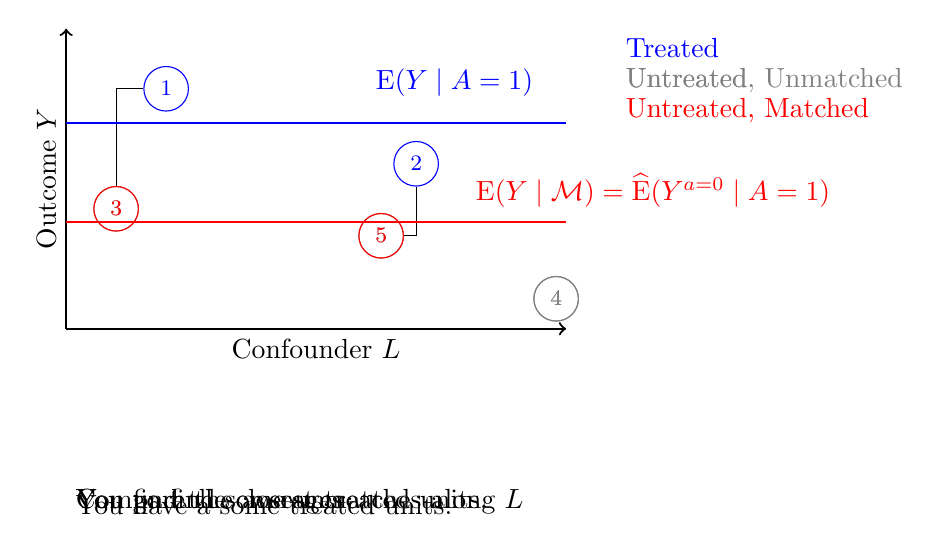
\begin{tikzpicture}[x = 2.5in, y = 1.5in]
\node at (0,-.3) {};
\draw[->, thick] (0,0) -- node[midway, below] {Confounder $L$} (1,0);
\draw[->, thick] (0,0) -- node[midway, above, rotate = 90] {Outcome $Y$} (0,1);
\node[anchor = north west, blue] at (1.1,1) {Treated};
\node[blue, draw, circle, font = \footnotesize] (p1) at (.2,.8) {$1$};
\node[blue, draw, circle, font = \footnotesize] (p2) at (.7,.55) {$2$};

\onslide<2-5>{
\node[anchor = north west, gray] at (1.1,.9) {Untreated};
\node[gray, draw, circle, font = \footnotesize] (p3) at (.1,.4) {$3$};
\node[gray, draw, circle, font = \footnotesize] (p4) at (.98,.1) {$4$};
\node[gray, draw, circle, font = \footnotesize] (p5) at (.63,.31) {$5$};
}
\draw<4-> (p3) |- node[pos = .75, left] {} (p1);
\draw<5-> (p5) -| node[pos = .75, right] {} (p2);
\node<1>[anchor = south west] at (0,-.65) {You have a some treated units.};
\node<2>[anchor = south west] at (0,-.65) {You go find some untreated units.};
\node<3-5>[anchor = south west, align = left] at (0,-.65) {You find the closest matches along $L$};
\onslide<6->{
\node[anchor = north west, gray] at (1.1,.9) {Untreated, Unmatched};
\node[anchor = north west, red] at (1.1,.8) {Untreated, Matched};
\node[red, draw, circle, font = \footnotesize] (p3) at (.1,.4) {$3$};
\node[gray, draw, circle, font = \footnotesize] (p4) at (.98,.1) {$4$};
\node[red, draw, circle, font = \footnotesize] (p5) at (.63,.31) {$5$};
}

\node<6->[anchor = south west] at (0,-.65) {Compare the averages };

\onslide<7>{
\draw[-, thick, red] (0,.355) -- node[right, below] {} (1,.355);
\draw[-, thick, blue] (0,.685) -- node[right, below] {} (1,.685);
\node[anchor = north west, red] at (.8,.55) {$\E(Y \mid \mathcal{M}) = \widehat{\E}(Y^{a =0} \mid A = 1)$};
\node[anchor = north west, blue] at (.6,.9) {$\E(Y \mid A = 1)$};

}
\end{tikzpicture}
\end{frame}

\begin{frame}{Why matching is great} \pause

\begin{enumerate}[<+->]
\item Completely transparent that $Y_i^1$ is observed
\item Easy to explain
\begin{itemize}
\item We had some treated units
\item We found a set of control units which are comparable
\item We compared the means
\end{itemize}
\item Can assess quality of matches before we look at the outcome
\item Model-free${}^*$
\begin{itemize}
\item ${}^*$ but you have to define what makes a match ``good''
\end{itemize}
\end{enumerate}

\end{frame}



\begin{frame}{Bias vs variance}
The idea of matching is straightforward, but the details matter!
\pause
\begin{figure}
    \centering
    \includegraphics[scale = .25]{Ch5/figures/bullseye.png}\footnote{Figure from: \url{http://scott.fortmann-roe.com/docs/BiasVariance.html}}
\end{figure}

\end{frame}

\begin{frame}{Matching in univariate settings: Algorithms}

\begin{itemize}
\item Caliper or no caliper
\item 1:1 vs $k$:1
\item With replacement vs without replacement
\item Greedy vs optimal
\end{itemize}

\end{frame}

\begin{frame}{Caliper or no caliper matching}

\centering
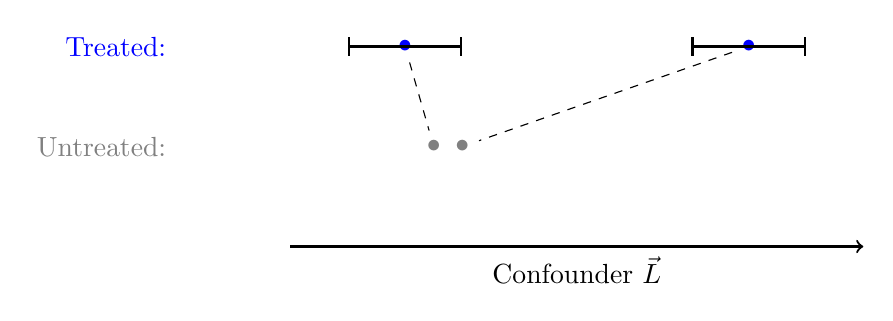
\begin{tikzpicture}[x = .6\textwidth, y = .5in]
\node[anchor = east, blue] at (-.2,1) {Treated:};
\node[anchor = east, gray] at (-.2,0) {Untreated:};
\node[blue] (p1) at (.2,1) {$\bullet$};
\node[gray] (p3) at (.25,0) {$\bullet$};
\onslide<1-5>{
\node[blue] (p2) at (.8,1) {$\bullet$};
\node[gray] (p4) at (.3,0) {$\bullet$};
}
\onslide<6->{
\node[blue, opacity = .1] (p2) at (.8,1) {$\bullet$};
\node[gray, opacity = .1] (p4) at (.3,0) {$\bullet$};
}
\draw[->, thick] (0,-1) -- node[midway, below] {Confounder $\vec{L}$} (1,-1);
\draw<2->[dashed] (p1) -- (p3);
\draw<3-5>[dashed] (p2) -- (p4);
\draw<6->[dashed, opacity = .1] (p2) -- (p4);
\draw<4->[|-|, thick] (.1,1) -- (.3,1);
\draw<4-5>[|-|, thick] (.7,1) -- (.9,1);
\draw<6->[|-|, thick, opacity = .1] (.7,1) -- (.9,1);
\end{tikzpicture}
\onslide<5->{
\begin{itemize}
\item Caliper: A radius around a treated unit such that we would rather drop the unit than make a match beyond that radius
\onslide<7->{
\item Feasible Sample Average Treatment Effect on the Treated (FSATT): Average among treated units for whom an acceptable match exists
}
\end{itemize}
}
\end{frame}

\begin{frame}{1:1 vs $k$:1 matching}

\centering
\begin{tikzpicture}[x = .6\textwidth, y = .5in]
\node[anchor = east, blue] at (-.2,1) {Treated:};
\node[anchor = east, gray] at (-.2,0) {Untreated:};
\node[blue] (p1) at (.2,1) {$\bullet$};
\node[gray] (p2) at (.25,0) {$\bullet$};
\node[gray] (p3) at (.3,0) {$\bullet$};
\node[blue] (p4) at (.8,1) {$\bullet$};
\node[gray] (p5) at (.76,0) {$\bullet$};
\node[gray] (p6) at (.81,0) {$\bullet$};
\draw[->, thick] (0,-1) -- node[midway, below] {Confounder $\vec{L}$} (1,-1);
\draw<2->[dashed] (p1) -- (p2);
\draw<2->[dashed] (p4) -- (p6);
\draw<3->[dashed] (p1) -- (p3);
\draw<3->[dashed] (p4) -- (p5);
\end{tikzpicture}
\onslide<4->{
\begin{itemize}
\item Benefit of 2:1 matching
\onslide<5->{
\begin{itemize}
\item Lower variance. Averaging over more cases.
\end{itemize}
}
\item Benefit of 1:1 matching
\onslide<6->{
\begin{itemize}
\item Lower bias. Only the best matches.
\end{itemize}
}
\onslide<7->{
\item Greater $k \rightarrow$ lower variance, higher bias
}
\end{itemize}
}
\end{frame}

\begin{frame}{With replacement vs without replacement matching}

\centering
\begin{tikzpicture}[x = .6\textwidth, y = .5in]
\node[anchor = east, blue] at (-.2,1) {Treated:};
\node[anchor = east, gray] at (-.2,0) {Untreated:};
\node[blue] (p1) at (.2,1) {$\bullet$};
\node[gray] (p2) at (.25,0) {$\bullet$};
\node[blue] (p3) at (.3,1) {$\bullet$};
\node[gray] (p4) at (.8,0) {$\bullet$};
\draw[->, thick] (0,-1) -- node[midway, below] {Confounder $\vec{L}$} (1,-1);
\draw<2->[dashed] (p1) -- (p2);
\draw<3->[dashed] (p3) -- node[midway, above] {?} (p4);
\draw<4->[dashed] (p3) -- node[midway, right] {?} (p2);
\end{tikzpicture}
\onslide<4->{
\begin{itemize}
\item Benefit of matching without replacement
\onslide<5->{
\begin{itemize}
\item Lower variance. Averaging over more cases.
\end{itemize}
}
\item Benefit of matching with replacement
\onslide<6->{
\begin{itemize}
\item Lower bias. Better matches.
\end{itemize}
}
\end{itemize}
}
\end{frame}

\begin{frame}{Greedy vs optimal matching\footnote{Gu, X. S., \& Rosenbaum, P. R. (1993). \bref{https://www.tandfonline.com/doi/abs/10.1080/10618600.1993.10474623}{Comparison of multivariate matching methods: Structures, distances, and algorithms.} Journal of Computational and Graphical Statistics, 2(4), 405-420.}}

\centering
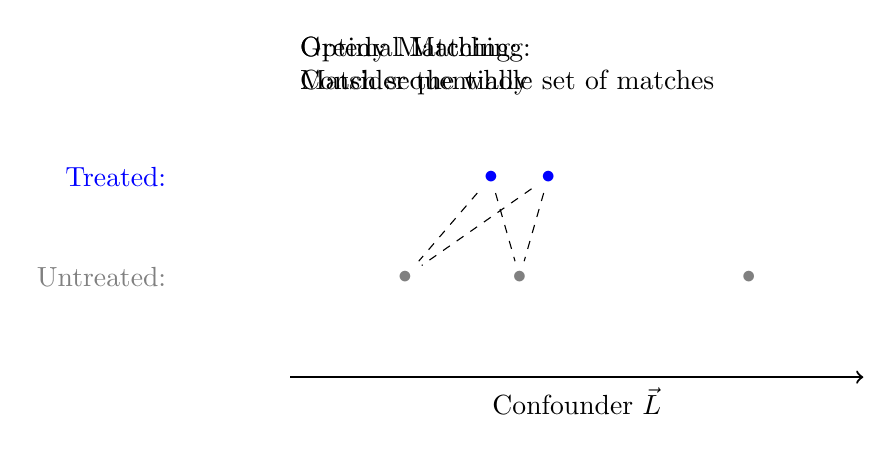
\begin{tikzpicture}[x = .6\textwidth, y = .5in]
\node[anchor = north west, align = left] at (0,2.5) {};
\node[anchor = east, blue] at (-.2,1) {Treated:};
\node[anchor = east, gray] at (-.2,0) {Untreated:};
\node[blue] (p1) at (.35,1) {$\bullet$};
\node[gray] (p2) at (.4,0) {$\bullet$};
\node[blue] (p3) at (.45,1) {$\bullet$};
\node[gray] (p4) at (.2,0) {$\bullet$};
\node[gray] (p5) at (.8,0) {$\bullet$};
\draw[->, thick] (0,-1) -- node[midway, below] {Confounder $\vec{L}$} (1,-1);
\node<2-4>[anchor = north west, align = left] at (0,2.5) {Greedy Matching:\\Match sequentially};
\draw<3-4>[dashed] (p1) -- (p2);
\draw<4-4>[dashed] (p3) -- (p4);
\node<5->[anchor = north west, align = left] at (0,2.5) {Optimal Matching:\\Consider the whole set of matches};
\draw<5->[dashed] (p1) -- (p4);
\draw<5->[dashed] (p3) -- (p2);
\end{tikzpicture}
\onslide<6->{
\begin{itemize}
\item Optimal is better. Just computationally harder.
\end{itemize}
}
\end{frame}

\begin{frame}{Matching in univariate settings: Algorithms}

\begin{itemize}
\item Caliper or no caliper
\item 1:1 vs $k$:1
\item With replacement vs without replacement
\item Greedy vs optimal
\end{itemize}

\pause
\vspace{1em}
Many reasonable choices, good choices depend on the data you have  

\end{frame}

\goalsframe

\end{document}